\documentclass{beamer}
\usepackage[utf8]{inputenc}
\usepackage[T1]{fontenc}
\usepackage{lmodern}
\usepackage[ngerman]{babel}
\usepackage{graphicx}
\usepackage{listings}
\usepackage{verbatim} % mainly for multi-line comments

\usetheme{Madrid}
\useinnertheme{rectangles}
\setbeamertemplate{navigation symbols}{}
\setbeamercovered{highly dynamic}

\title{Tracking juggling balls using the Kinect}
\author[Rolf $\cdot$ Thiemo $\cdot$ Flo]{Rolf Boomgaarden $\cdot$ Thiemo Gries $\cdot$ Florian Letsch}
\institute{Universität Hamburg}
\date{30. Mai 2013}

\begin{document}

\frame
{
\titlepage
}

\begin{frame}{A juggling robot}

\textbf{Playing Catch and Juggling with a Humanoid Robot}
Jens Kober$^{1}$, Matthew Glisson, and Michael Mistry$^{2}$

Disney Research, Pittsburgh, USA

$^{1}$ Bielefeld University, Germany

$^{2}$ University of Birmingham, UK

\begin{center}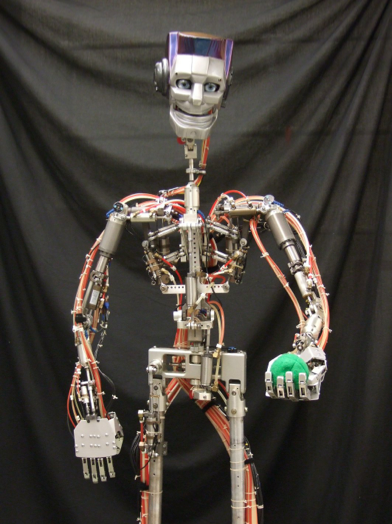
\includegraphics[width=4cm]{img/robot.png}\end{center}
   
\end{frame}

\frame
{
\tableofcontents
}

\section{A Juggling Robot}


\begin{frame}{System description}
\begin{enumerate}
\item Robot hardware
\item Vision system
\item Ball Filtering and Prediction
\item Robot State Machine
\item Catching Algorithm
\item Throwing Approach
\item Juggling
\end{enumerate}
\end{frame}

\begin{frame}{Image processing pipeline}
\begin{center}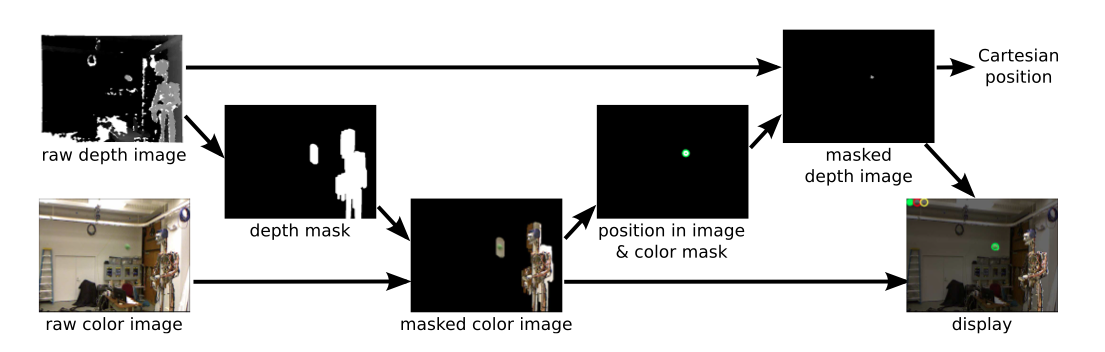
\includegraphics[width=12cm]{img/img-processing.png}\end{center}
\end{frame}


\section{Hough Transform}

\begin{frame}{Hough Transform}
\begin{center}
\includegraphics<1-1>[scale=1]{img/Hough1.png}
\includegraphics<2-2>[scale=1]{img/Hough2.png}
\includegraphics<3-3>[scale=1]{img/Hough3.png}
\end{center}
\end{frame}

\section{Kalman Filter}

\begin{frame}{Kalman Filter}
\begin{itemize}
\item nutzt verschiedene Daten, um den aktuellen Zustand zu schätzen:
\begin{itemize}
\item Daten aus Wissen über die Zustandsänderung
\item Sensordaten
\end{itemize}
\item kann mit diesen auch zukünftige Zustände schätzen
\end{itemize}
\end{frame}

\begin{frame}{Kalman Filter}{Anwendungsfall}
\begin{center}
\includegraphics<1-1>[scale=0.45]{img/kalman_0_1.jpg}
\includegraphics<2-2>[scale=0.45]{img/kalman_0_2.jpg}
\includegraphics<3-3>[scale=0.45]{img/kalman_0_3.jpg}
\includegraphics<4-4>[scale=0.45]{img/kalman_0_4.jpg}
\end{center}
\end{frame}

\begin{frame}{Kalman Filter}{Formeln}
\begin{itemize}
\item<1-> predict
\begin{itemize}
\item<2-> mit Wissen über die Art der Bewegung wird eine voraussichtliche Position berechnet:\\\qquad\qquad$\overline{x}_{t} = A_{t}x_{t-1} + B_{t}u_{t} + \varepsilon_{t}$
\item<2-> zusätzlich werden die Sensordaten (hier GPS) geschätzt:\\\qquad\qquad$\overline{z}_{t} = H_{t}\overline{x}_{t} + \varepsilon_{t}$
\end{itemize}
\item<1-> update
\begin{itemize}
\item<3-> geschätzte Positionen werden mit Sensordaten korrigiert:\\\qquad\qquad$x_{estimate} = \overline{x}_{t} + K(z_{t} - \overline{z}_{t})$
\end{itemize}
\end{itemize}
\end{frame}

\begin{frame}{Kalman Filter}{Unsere Anwendung}
\begin{itemize}
\item Wissen über Art der Bewegung $\rightarrow$ Wurfparabel
\item Sensordaten $\rightarrow$ Kinect
\end{itemize}
\end{frame}

\begin{frame}{Conclusion}
	\begin{itemize}
	\item 75\% success in feasable catching region
	\item 47\% overall catching
	\pause \item Video
	\end{itemize}
	
\end{frame}


\section{Our plan}
\begin{frame}{The flow}
\begin{center}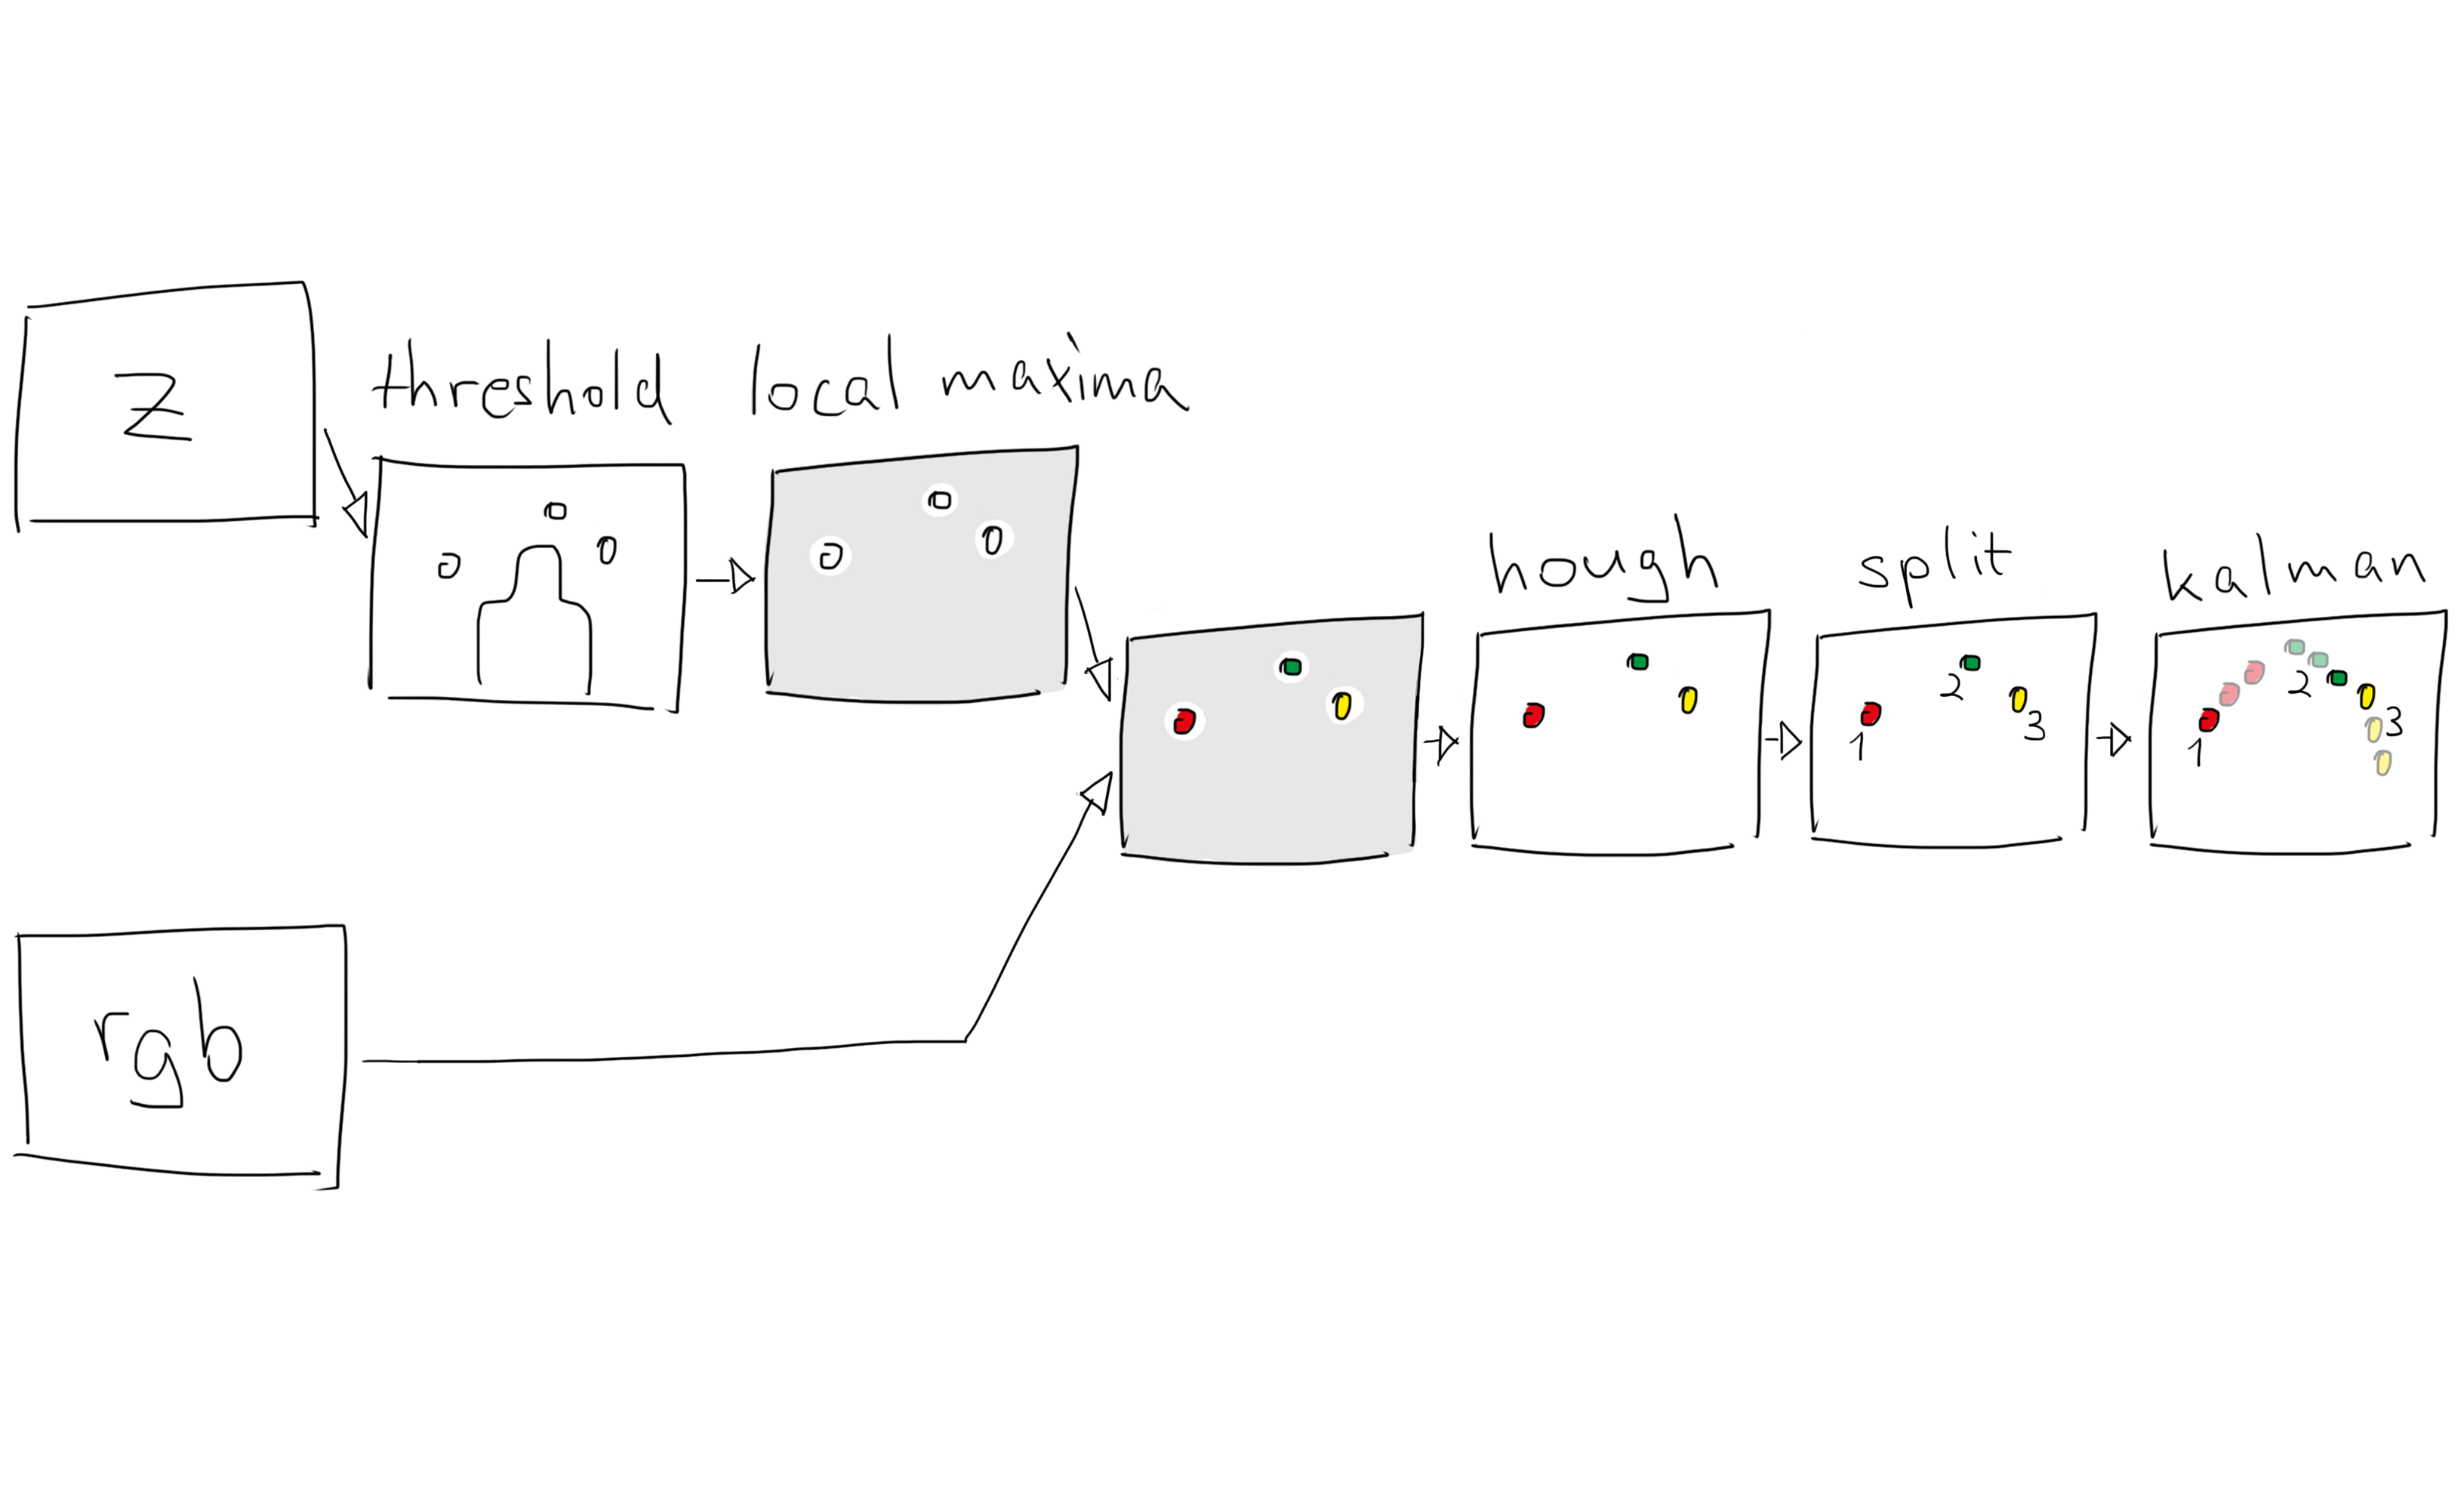
\includegraphics[scale=0.1045]{img/flowchart.png}\end{center}
\end{frame}

\begin{frame}{Challenges}
\begin{itemize}
	\item Local maxima
	\item Multiple balls (colour?)
\end{itemize}
\end{frame}

\begin{frame}{The end}
EOF
\end{frame}

\end{document}






